\section{Co-design of Computation and Control for Autonomous Systems}
\subsection{Motivation}

Real-time control of autonomous vehicles requires the processing of a large amount of sensor data from cameras, LIDAR, radars, encoders, inertial sensors and possibly information communicated by other vehicles or the road infrastructure.
This data is used by the vehicle to determine its position in the world and that of neighboring obstacles, which we refer to as \emph{state estimation}, and to calculate its next move.
Google's autonomous vehicles generate over 750MB/s of sensor data \cite{diamandis2015bold} which must be processed by the perception pipeline fast enough for timely control decisions.
The perception pipeline uses \emph{run-to-completion} algorithms: such algorithms must always meet a pre-defined termination criterion before returning a useful answer.
If interrupted early, they don't return anything useful to the controllers.
Typical algorithms in a perception pipeline span tasks like edge detection, filtering, segmentation, object recognition and tracking, and sensor fusion. 
 
Perception algorithms have variable execution times because their runtimes depend on the current context.
E.g., a corner detector will take longer to detect all the corners in a rich scene than in a flat homogeneous scene (at a given processor frequency).
Because of this variability, the hardware running these run-to-completion algorithms is over-engineered for the worst-case execution time.
That is, the system is equipped with hardware that can always execute the software within a certain deadline.
When the current context causes the perception pipeline to perform the most operations (e.g., the corner detector has to find many corners), this is appropriate.
However, such worst-case situation rarely holds in practice. 
The rest of the time, the perception pipeline has fewer operations to perform within the deadline, so a slower (and less power-hungry) hardware execution would be appropriate.
The downside with this over-engineering is unnecessarily large power consumption for the average case.
For example, in many research autonomous vehicles, this leads to a requirement of up to 4KW in computational power \cite{powerNagoya}. 
This is a significant drain on the vehicle's lithium-ion battery capacity, which is 24kWh in a Nissan Leaf, for example.
It is also a significant compared to the average power drawn by the drive motors, which is around 3KW in a small electric vehicle modeled in ADVISOR \cite{nreladvisor} going through the Urban Dynamometer Drive Cycle. 
%%\mynote{HA}{30kW is peak, no?}
%%\mynote{YP}{Yes, good point, corrected. Also changed over 4KW to upto 4KW, don't want to claim too much esp. since we do not have concrete data on it. And please check the private communication citation for it.}

In addition to the high power consumption, the rigid nature of the run-to-completion algorithms used for perception and state estimation restricts the range of maneuvers that autonomous systems can do, e.g. autonomous cars are not yet capable of fast or aggressive driving.
Reacting faster to a dynamic scene requires a perception pipeline (and state estimation) that can deliver answers faster, even if the cost is slightly worsened quality of output.

\subsection{Challenge}
The challenge is to enable less power-hungry autonomous vehicles that still maintain the \emph{control performance} of current systems.
Note that the emphasis is on control performance, and not on the output quality of the perception algorithm.
While in general, the two are positively correlated (better output quality means better control performance) there are situations where this is not the case.
For example, if the lower quality output is produced faster, allowing a faster update of the control input.

From the above discussion it can be seen that we ought to design control algorithms that recognize how soon an update is needed from the perception and state estimation (P\&SE) pipeline. 
Correspondingly, we should also design P\&SE  algorithms that can provide useful answers even when interrupted before their run-to-completion criterion has been met. 
The main challenges in such a system are:
\begin{itemize}
\item Enabling common perception algorithms to provide useful (if lower quality) answers early.
This is a challenging task for any given algorithm as they are most often designed and implemented for maximum performance without consideration for the possibility of interruption.
\item Development of control/scheduling algorithms that are aware of when to request faster updates for the optimal operation of the closed loop system.
Existing work models the effect of delays on control and designs controllers that operate well despite the delay.
Here we are suggesting that rather than view the delays as purely adversarial, the controller should be aware of the range of trade-offs afforded it by the P\&SE algorithms and exploit these trade-offs for lower-power control. 
\end{itemize}
\begin{figure}[!b]
	\centering
	\vspace{-20pt}
	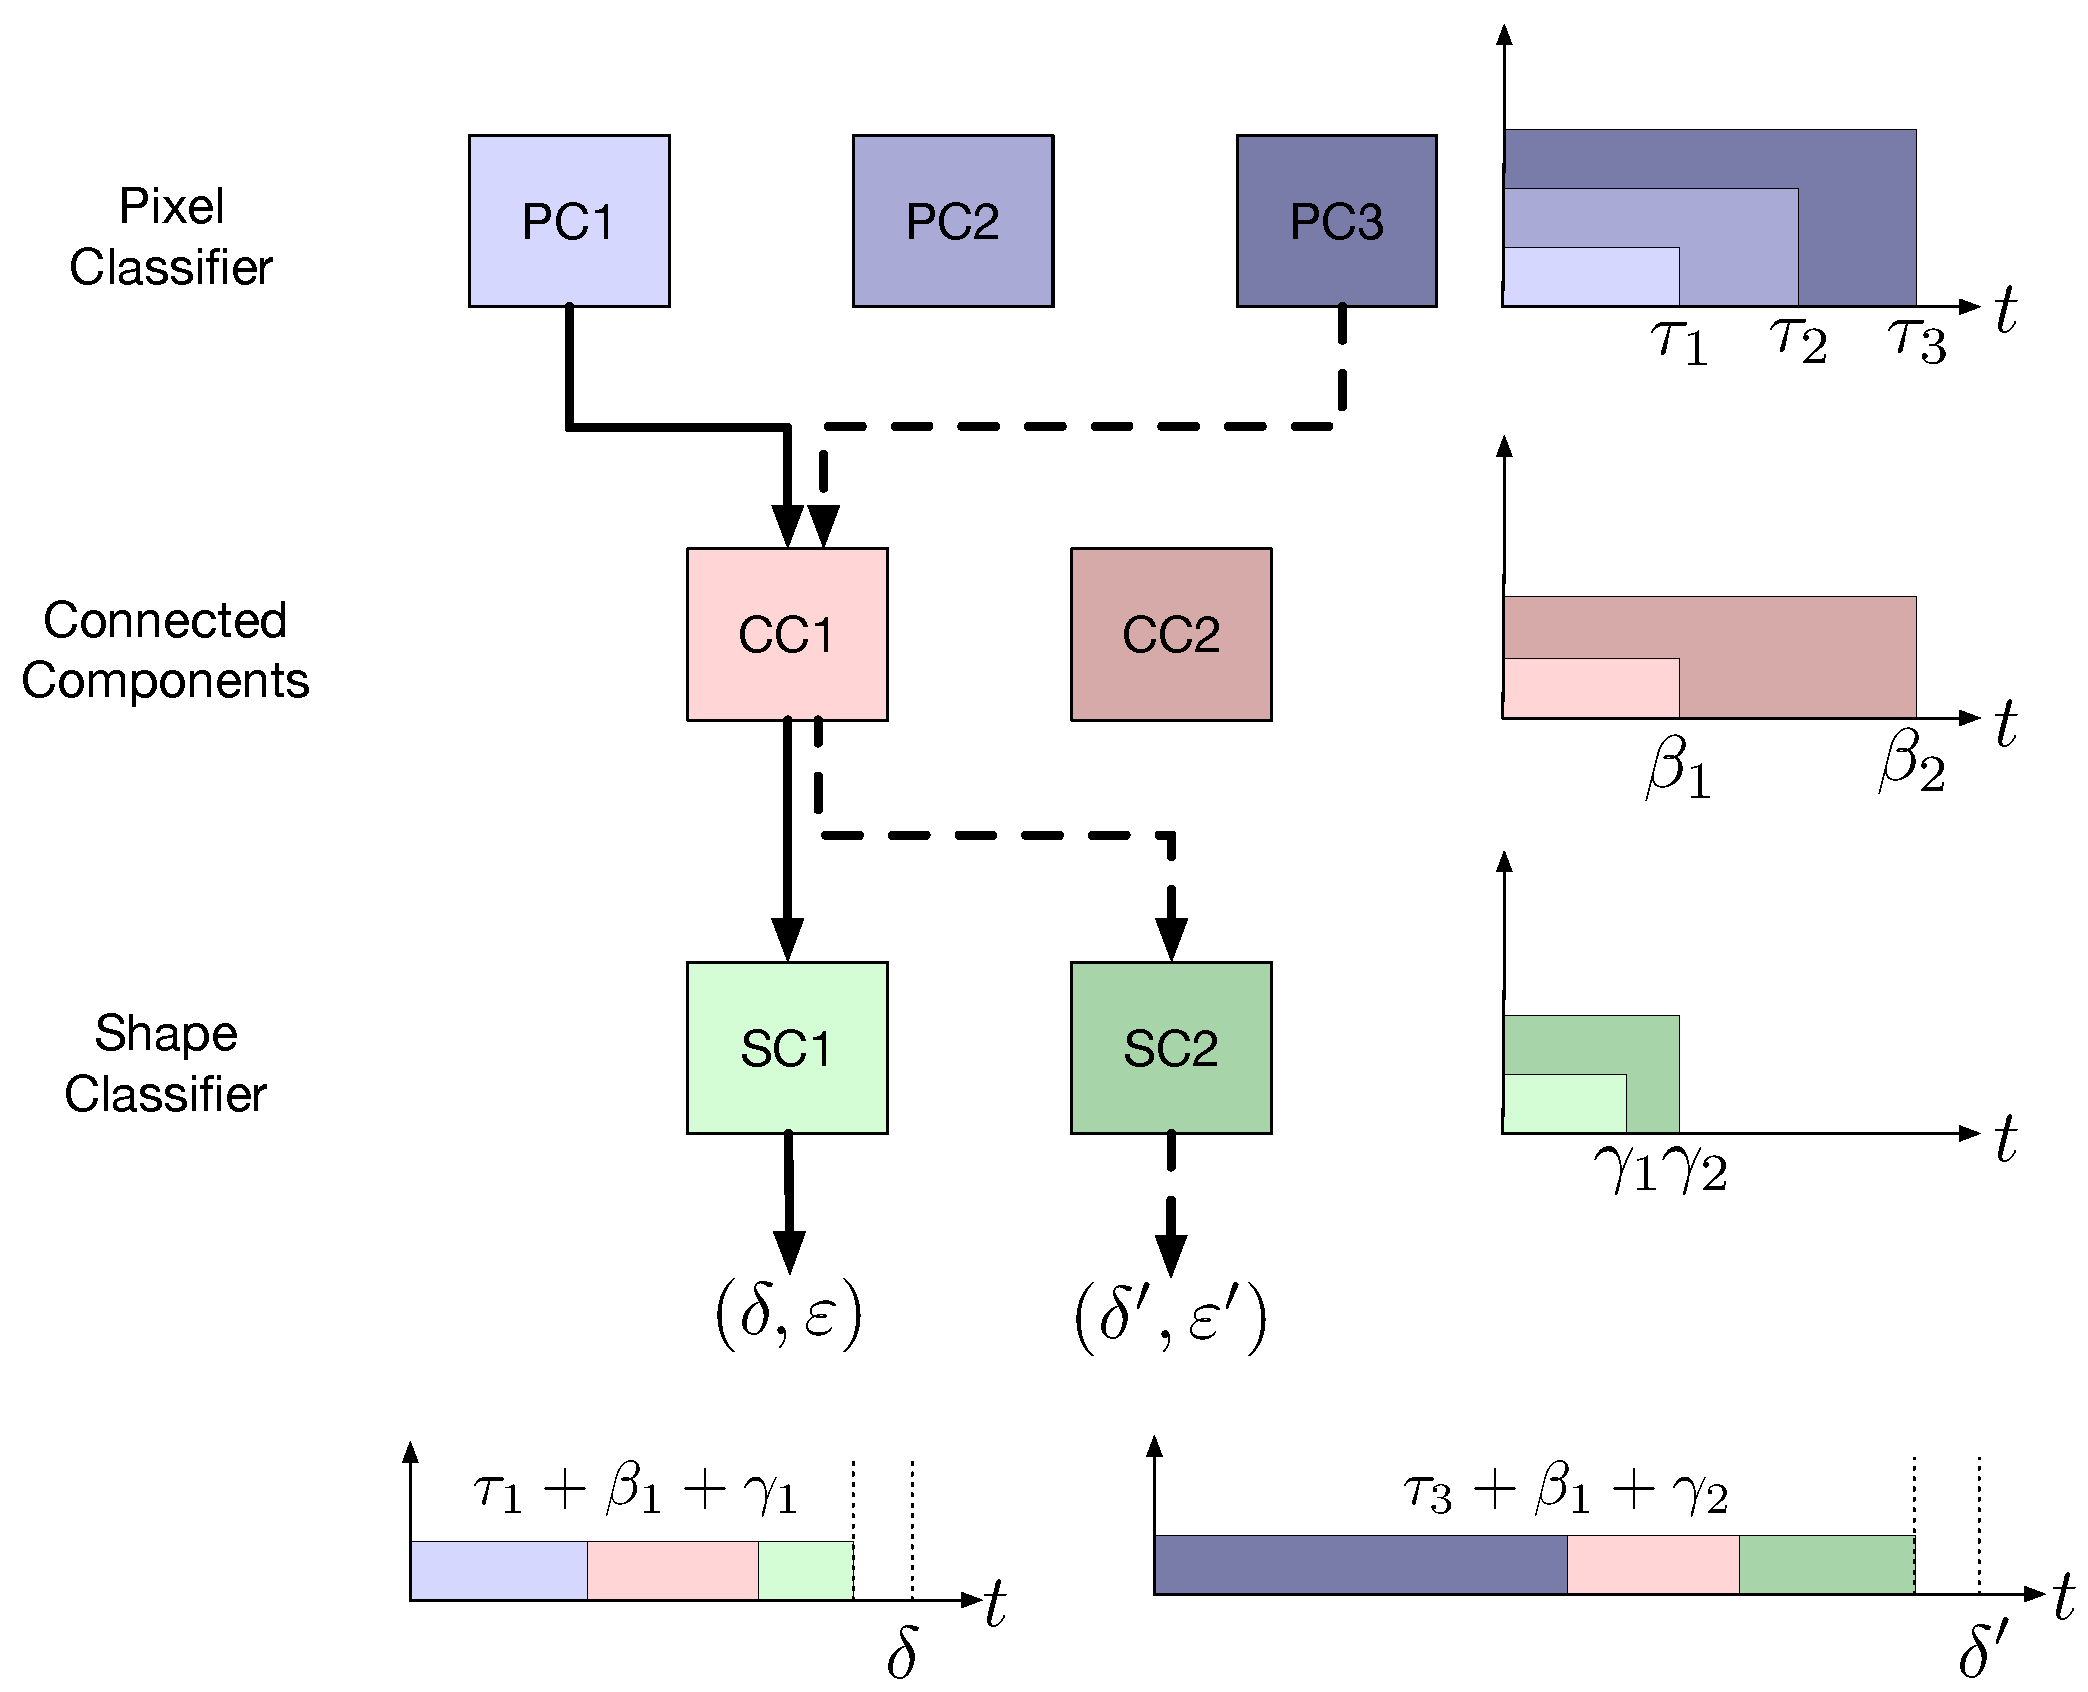
\includegraphics[width=0.49\textwidth]{Figures/real_time_figure.pdf}
	\caption{A perception algorithm for object detection is decomposed into three tasks, and various components used to compose the contract based perception algorithm and their representation as real-time tasks. For a given $\delta$ contract, knob settings are chosen at run-time resulting in a schedule to execute these sequential components, or tasks, to respect the contract. }
	\label{fig:offline}
\end{figure}

\subsection{Contract-based Co-design of Anytime Computation and Robust Control}
Anytime algorithms \cite{boddy} are a class of algorithms that can be interrupted at any point during their execution and still return a usable solution, usually one whose quality is monotonically improving with time. 
\emph{Contract algorithms} \cite{zilbersteinAImag} are a version of anytime algorithms where the interruption time is chosen from a set of pre-defined times. 
%The use of such algorithms for the computationally heavy perception and estimation algorithms would give a level of flexibility with a computation time/quality trade-off that is not offered by run-to-completion algorithms. In general, most perception and estimation algorithms do not lend themselves to such implementations.
In our recent work \cite{RTSS15, Complex15}, we show how to convert off-the-shelf P\&SE algorithms into \emph{contract algorithms}, and how to design a controller that takes advantage of this capability.

%\mynote{HA}{Way too contrived, Yash...say things more plainly, in the active voice. The next paragraph doesn't actually give any information, it's a string of words. Example: what does "realization" mean? testing? design? implementation? analysis? if there's a more precise word, use it. if there isn't, explain what you mean by it.}
\begin{figure}[t]
	\centering
	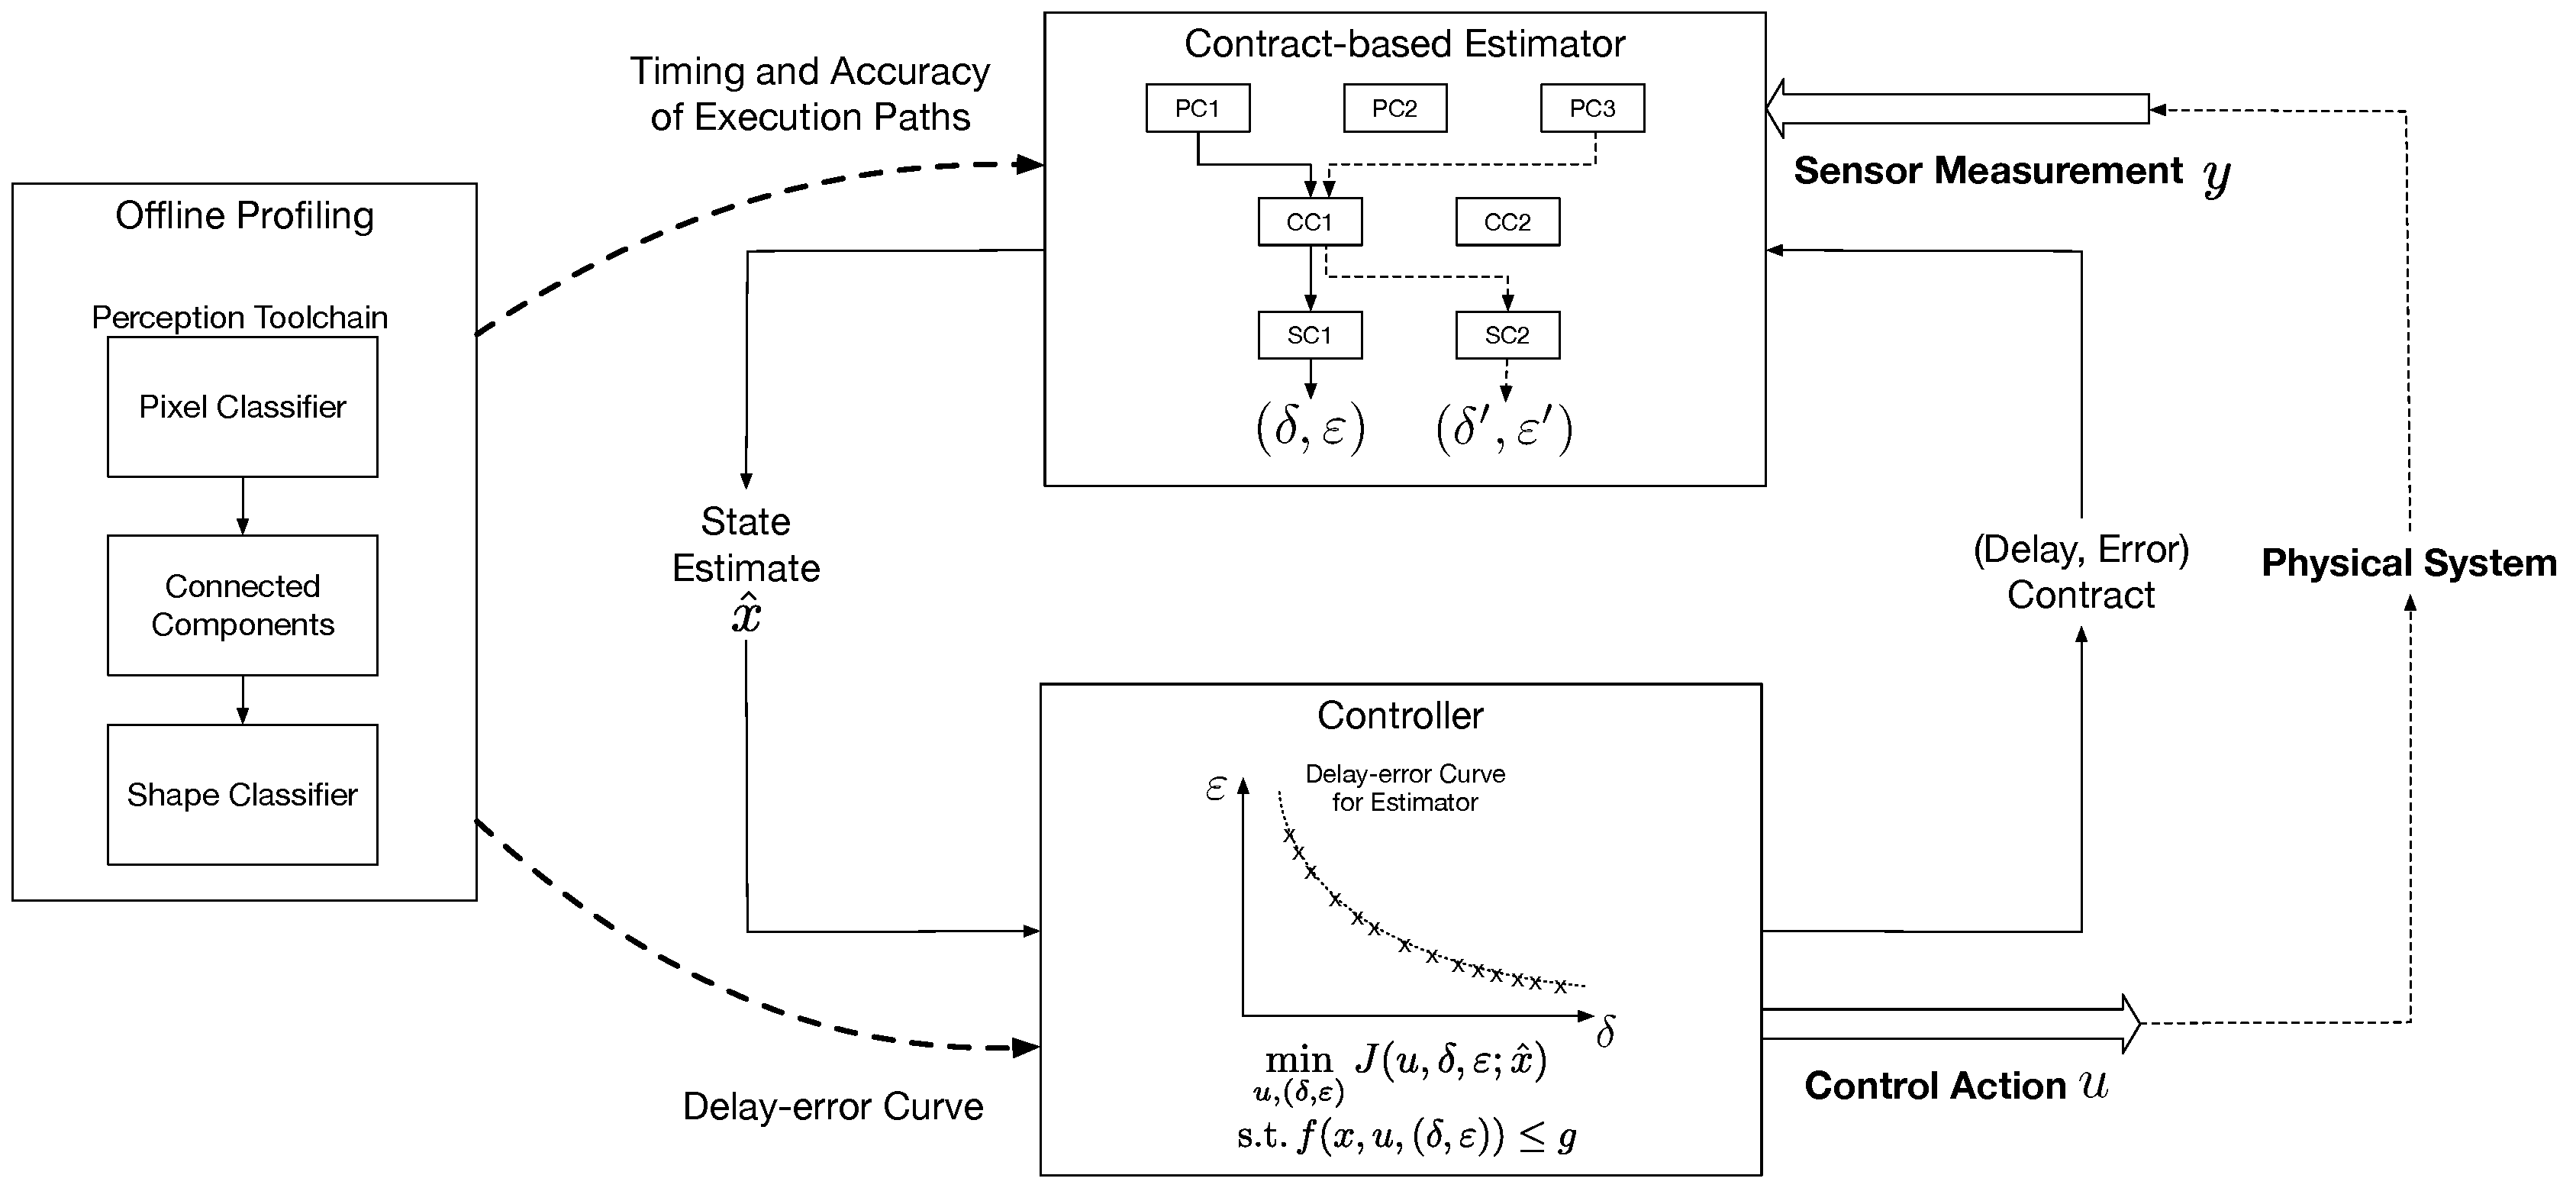
\includegraphics[width=0.49\textwidth]{Figures/process_figure2.pdf}
	\caption{Contract-based estimator and controller. This differs from regular state-estimation based feedback control as the controller can set contracts (deadlines) for the perception/estimation algorithm. Based on the contract and the offline profiling, the contract based estimator decides at run-time what tasks to execute in order to best meet the contract.}
	\label{fig:fullcodesignedCE}
	\vspace{-10pt}
\end{figure}

First, the PS\&E is profiled off-line.
Namely, the algorithm's parameters are varied and for each setting of the parameters, it is run on a \emph{profiling data set}. 
This yields a finite set of \emph{contracts}: a contract is a pair (estimation delay, estimation error), and each setting of the parameters yields one contract when run on the profiling data set
Fig. \ref{fig:offline} shows this approach applied to an object detection algorithm.
At run-time, when the estimator receives a (delay, error) contract request from the controller, it can adapt its execution paths to respect the contract, namely, to provide a state estimate within the requested error bound, and within the requested delay.
Another dimension of decision making, explored in \cite{Complex15}, is resource allocation for execution of tasks, e.g. whether the task gets executed on the CPU or the GPU, resulting in a power versus computation delay trade-off.

The controller is designed with the knowledge of the contracts that can be realized by the P\&SE algorithm, and at each time step will request a contract.
This gives the controller the ability to leverage the flexible nature of the estimation algorithm to maximize some measure of control performance. %\todo[inline]{Might want to avoid mentioning \emph{separability principle}}
In \cite{RTSS15} we develop a Robust Model Predictive Control algorithm that can leverage this trade-off offered by the contract based co-design (see Fig. \ref{fig:fullcodesignedCE} while optimizing for a joint cost of control performance and computation power consumption. We experimentally evaluated our approach on a hex-rotor with visual odometry and showed improved control performance and computation energy efficiency over a baseline MPC controller that does not leverage co-design.


Fig.~\ref{fig:fullcodesignedCE} shows the closed loop architecture in a system with co-design of the anytime computation (estimator) and robust controller.
In the co-designed system as presented in this paper, the controller can make the estimation algorithm switch to lower or higher time (and/or energy) consuming modes based on the control objective at the current time step.
The main components of the co-design architecture are a contract based perception-and-estimation algorithm, a robust control algorithm that computes an input to be sent to the physical system being controller as well as the operating mode for the contract time estimator, and the interface between them. More details on these components are in the following sections.




